% TU Delft beamer template
% Author: Erwin Walraven (initial version was created by Maarten Abbink)
% Delft Universiy of Technology

\documentclass{beamer}
\usepackage[english]{babel}
\usepackage{calc}
\usepackage[absolute,overlay]{textpos}
\usepackage{graphicx}
\usepackage{subcaption}
\captionsetup[figure]{font=scriptsize,labelfont=scriptsize}
\captionsetup[subfigure]{font=scriptsize,labelfont=scriptsize}
\usepackage{amsmath}
\usepackage{amsfonts}
\usepackage{amsthm}
\usepackage{mathtools}
\usepackage{comment}
\usepackage{MnSymbol,wasysym}

\setbeamertemplate{navigation symbols}{} % remove navigation symbols
\mode<presentation>{\usetheme{tud}}

% BIB SETTINGS
%\usepackage[backend=bibtex,firstinits=true,maxnames=30,maxcitenames=20,url=false,style=authoryear]{biblatex}
%\bibliography{bibfile}
%\setlength\bibitemsep{0.3cm} % space between entries in the reference list
%\renewcommand{\bibfont}{\normalfont\scriptsize}
%\setbeamerfont{footnote}{size=\tiny}
%\renewcommand{\cite}[1]{\footnote<.->[frame]{\fullcite{#1}}}


\title[]{Transiently-powered Battery-free Robot}
\institute[]{Delft University of Technology}
\author{Koen Schaper}
\date{15 December 2017}

\logo{\includegraphics[width=3cm]{pics/es_logo_cyan_black_rgb}}

\begin{document}
{
\setbeamertemplate{footline}{\usebeamertemplate*{minimal footline}}
\frame{\titlepage}
}

{\setbeamertemplate{footline}{\usebeamertemplate*{minimal footline}}

}

\begin{comment}
\begin{frame}{Overview}
		Introduction \\
		\vspace{1em}
		Design and Implementation
		\begin{itemize}
			\item Hardware
			\item Control software
		\end{itemize}
		\vspace{1em}
		Evaluation \\
		\vspace{1em}
		Conclusion
\end{frame}
\end{comment}

\begin{frame}{Small robotic platforms}
	\textbf{Future applications}
	\begin{itemize}
		\item Search and rescue
		\item Exploration
	\end{itemize}
	\pause
	\begin{figure}
		\centering
		\begin{subfigure}[b]{0.28\textwidth}
			\includegraphics[width=\textwidth]{pics/zooids.jpg}
			\caption*{Zooids}
		\end{subfigure}
		\quad
		\begin{subfigure}[b]{0.2825\textwidth}
			\includegraphics[width=\textwidth]{pics/rovables.jpg}
			\caption*{Rovables}
		\end{subfigure}
		\quad
		\begin{subfigure}[b]{0.2815\textwidth}
			\includegraphics[width=\textwidth]{pics/toio.jpg}
			\caption*{Sony Toio}
		\end{subfigure}
	\end{figure}
	\pause
	\textbf{Problem:} Operation time is limited by Lithium-ion batteries
\end{frame}

\begin{frame}{Problem of batteries}
	\begin{minipage}{0.54\textwidth}
		\textbf{New battery technologies}
		\begin{itemize}
			\item Overhyped and slow emerging
		\end{itemize}
		\vspace{0.5em}
		\textbf{Replenishment methods}
		\begin{itemize}
			\item Recharging or battery replacement
		\end{itemize}
	\end{minipage}
	\begin{minipage}{0.45\textwidth}\raggedleft
		\begin{figure}
			\centering
			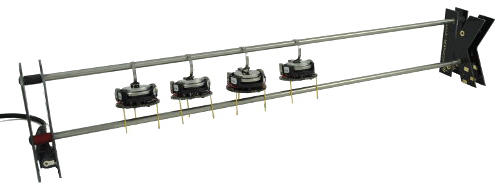
\includegraphics[width=0.9\textwidth]{pics/Kilobot_charger_with_robots1-495x188.png}
		\end{figure}
	\end{minipage} \\
	\vspace{3em}
	\pause
	\textbf{Solution:} 
	Energy from ambient sources stored in capacitors
\end{frame}

\begin{frame}{Energy harvesting}
	%\vspace{1em}
	\begin{figure}
		\centering
		\includegraphics[width=0.8\textwidth]{pics/Harvesting-diagram.png}
	\end{figure}
	%\pause
	\begin{minipage}{0.45\textwidth}
		\textbf{1000x} smaller energy storage \\\\\\
		\textbf{Challenge}: \\
		Frequent power interrupts
	\end{minipage}
	\begin{minipage}{0.54\textwidth}\raggedleft
		\begin{figure}
			\vspace{2em}
			\includegraphics[width=0.9\textwidth]{pics/Voltage_time_harvester.png}
			\caption*{Image: Naderiparizi RFID' 15}
		\end{figure}
	\end{minipage}
\end{frame}

\begin{frame}{Research question}
	\begin{center}
	%\begin{block}{}
		\textbf{What is the effect of intermittency on the movement accuracy of a transiently-powered robot without external feedback?}
	%\end{block}	
	\end{center}
\end{frame}

\begin{frame}{Design requirements}
	\textbf{Power} \\
	\begin{itemize}
		\item Not rely on batteries
	\end{itemize}
	\textbf{Small form factor} \\
	\begin{itemize}
		\item Lower material cost
	\end{itemize}
    \textbf{Locomotion} \\
    \begin{itemize}
    	\item Efficient actuator for movement
    \end{itemize}
    \textbf{Controlled movements} \\
    \begin{itemize}
    	\item Complete movement across power cycles
    \end{itemize}
\end{frame}

\begin{comment}
\begin{frame}{Power}
	\vspace{1em}
	\begin{minipage}{0.45\textwidth}
		Energy from light \\
		
		Solar panel \\
		
		\textbf{6\,s} Charge time \\
		
		\textbf{1\,s} Operation time \\
		
	\end{minipage}
	\begin{minipage}{0.54\textwidth}\raggedleft
		\begin{figure}
			\includegraphics[width=0.9\textwidth]{pics/light_setup.jpg}
			\caption*{Light setup}
		\end{figure}
	\end{minipage}
\end{frame}
\end{comment}

\begin{comment}
\begin{frame}{Locomotion}
	\begin{minipage}{0.45\textwidth}
		Geared DC motors \\
		
		Start current peak \\
		
		Maximum current harvester: \\
		110\,mA
	\end{minipage}
	\begin{minipage}{0.54\textwidth}\raggedleft
		\begin{figure}
			\includegraphics[width=\textwidth]{pics/free_running_current.png}
			\caption*{DC motor current profile}
		\end{figure}
	\end{minipage} \\
	\pause
	\vspace{1em}
	\textbf{Solution:} Pulse Width Modulation + Bulk capacitor
\end{frame}
\end{comment}

\begin{frame}{Schematic overview}
	\begin{figure}
		\centering
		\includegraphics[width=0.9\textwidth]{pics/schematic_robot_v2.png}
	\end{figure}
\end{frame}

\begin{frame}{Robot implementation}
	\begin{figure}
		\centering
		\includegraphics[width=0.9\textwidth]{pics/tp_robot2.png}
	\end{figure}
\end{frame}

\begin{frame}{PCB implementation}
	\vspace{1em}
	\begin{figure}
		\centering
		\begin{subfigure}[b]{0.35\textwidth}
			\includegraphics[width=\textwidth]{pics/pcb_front.jpg}
			\caption*{Front side}
		\end{subfigure}
		\qquad
		\begin{subfigure}[b]{0.35\textwidth}
			\includegraphics[width=\textwidth]{pics/pcb_back.jpg}
			\caption*{Back side}
		\end{subfigure}
	\end{figure}
\end{frame}


\begin{frame}{Motion control}
	\begin{minipage}{0.45\textwidth}
		Straight and curved movements\\
		
		Yaw-rate from gyroscope \\
		
		PID controller \\
		
		Movement target \\
		
		Persistent checkpoints\\
	\end{minipage}
	\pause
	\begin{minipage}{0.54\textwidth}\raggedleft
		\begin{figure}
			\centering
			\includegraphics[width=0.8\textwidth]{pics/Flowchart_code.png}
		\end{figure}
	\end{minipage}
\end{frame}

\begin{comment}
\begin{frame}{PID controller}
The controller periodically tries to reduce the yaw error as \\

\begin{equation}
e(t) = \psi_{\text{target}} - \psi(t),
\end{equation} \\
\vspace{1em}
\noindent
where $\psi_{\text{target}}$ is the yaw-rate target and $\psi(t)$ the yaw-rate obtained by the gyroscope. \\
\vspace{1em}
The PID controller adjusts its output as \\

\begin{equation}
u(t) = K_{\text{p}}e(t) + K_{\text{i}} \int_{0}^{t}e(\tau)d\tau + K_{\text{d}}\frac{d}{dt}e(t),
\end{equation} \\
\vspace{1em}
\noindent
where $K_{p}$, $K_{i}$ and $K_{d}$ are the tunable gains.
\end{frame}

\begin{frame}{Tuning PID controller}
	\begin{figure}
		Ziegler-Nichols Closed-Loop Tuning Method
		\begin{center}
		\begin{subfigure}[b]{0.49\textwidth}
			\includegraphics[width=\textwidth]{pics/straight_ku.png}
			\caption*{Determining the ultimate gain}
		\end{subfigure}
		\begin{subfigure}[b]{0.49\textwidth}
			\includegraphics[width=\textwidth]{pics/straight_ku_with_tu.png}
			\caption*{Result of applying the gains}
		\end{subfigure}
		\end{center}
	\end{figure}
\end{frame}
\end{comment}

\begin{frame}{Evaluation}
	Determine the accuracy of movement
	\pause
	\vspace{1em}
	\begin{figure}
		\centering
		\begin{subfigure}[b]{0.45\textwidth}
			\includegraphics[width=\textwidth]{pics/movement_setup.jpg}
			\caption*{Camera setup}
		\end{subfigure}
		\quad
		\begin{subfigure}[b]{0.45\textwidth}
			\includegraphics[width=\textwidth]{pics/movement_example.png}
			\caption*{Tracking with OpenCV}
		\end{subfigure}
	\end{figure}
	%Artificial power interrupts
\end{frame}

\begin{frame}{Solar powered demo}
\begin{figure}
	\centering
	\includegraphics[width=\textwidth]{pics/video.jpg}
\end{figure}
\end{frame}

\begin{frame}{Minimum on time}
	\vspace{0.5em}
	%4\,s straight movements
	\vspace{-0.5em}
	\begin{figure}
		\centering
		\begin{subfigure}[b]{0.28\textwidth}
			\includegraphics[width=\textwidth]{pics/figure_40.png}
			\caption*{Duty cycle 40\%}
		\end{subfigure}
		\hspace{2em}
		\begin{subfigure}[b]{0.28\textwidth}
			\includegraphics[width=\textwidth]{pics/figure_90.png}
			\caption*{Duty cycle 90\%}
		\end{subfigure}
	\end{figure}
	\pause
	\vspace{0.5em}
	\textbf{Conclusion 1:} Minimum on time $\geq$ 0.3\,s \\
	\textbf{Conclusion 2:} Speed decrease due to power interrupts \\
\end{frame}

\begin{frame}{Straight movements}
	\vspace{0.5em}
	%Average speed experimentally determined
	\vspace{-0.5em}
	\begin{figure}
		\centering
		\begin{subfigure}[b]{0.28\textwidth}
			\includegraphics[width=\textwidth]{pics/straight_40.png}
			\caption*{Duty cycle 40\%}
		\end{subfigure}
		\hspace{2em}
		\begin{subfigure}[b]{0.28\textwidth}
			\includegraphics[width=\textwidth]{pics/straight_90.png}
			\caption*{Duty cycle 90\%}
		\end{subfigure}
	\end{figure}
	\pause
	\vspace{0.5em}
	\textbf{Conclusion 1:} Interrupts increase horizontal deviation \\
	\textbf{Conclusion 2:} Solar powered more stable \\
\end{frame}

\begin{frame}{Circular movements}
	\vspace{-1em}
	\begin{figure}[h!]
		\centering
		\begin{subfigure}[b]{0.49\textwidth}
			\includegraphics[width=\textwidth]{pics/circle_40.png}
			\caption*{Duty cycle 40\%}
		\end{subfigure}
		\begin{subfigure}[b]{0.49\textwidth}
			\includegraphics[width=\textwidth]{pics/circle_90.png}
			\caption*{Duty cycle 90\%}
		\end{subfigure}
	\end{figure}
	\pause
	\vspace{0.5em}
	\textbf{Conclusion:} Higher duty cycle decreases deviation from circular path
\end{frame}

\begin{frame}{Conclusion}
	%16\% power duty cycle \\
	%\vspace{1em}
	\textbf{Minimum on time} \\
	\begin{itemize}
		\item Required for linear motion control
	\end{itemize}
	\vspace{1em}
	\textbf{Transiently-powered vs battery-powered robot} \\
	\begin{itemize}
		\item No significant differences in accuracy of movement
	\end{itemize}
	\vspace{1em}
	\textbf{Transiently-powered robot is feasible} \\
	\begin{itemize}
		\item Potential for self-sufficient and energy-autonomous robots
	\end{itemize}
\end{frame}

\begin{frame}{Future Work}

	\textbf{Speed feedback} \\
	\begin{itemize}
		\item Local sensing or external feedback
	\end{itemize}
	\textbf{Communication} \\
	\begin{itemize}
		\item Backscatter communication channel from the WISP
	\end{itemize}
	\textbf{Transiently-powered swarm} \\
	\begin{itemize}
		\item Swarm behavior with collective of transiently-powered robots
	\end{itemize}
	\textbf{Size reduction} \\
	\begin{itemize}
		\item Reduce cost and energy required for movement
	\end{itemize}
	\textbf{Sensing capabilities} \\
	\begin{itemize}
		\item Additional sensors for future applications
	\end{itemize}
	
\end{frame}

\begin{frame}{}
	\begin{center}
		\textbf{\huge{Questions?}}
		\vspace{2em}
		\begin{figure}
			\includegraphics[width=0.8\textwidth]{pics/tp_robot.png}
		\end{figure}
	\end{center}
\end{frame}

\end{document}
